\chapter{Method}

In this section, we introduce the level set method and dynamic implicit surfaces. Their role in segmentation is discussed having introduced having defined mathematical constructs such as signed distance transforms.

\section{Level Set Method}\label{levelsetmethod}
The level set method evolves a contour (in two dimensions) or a surface (in three dimensions) implicitly by manipulating a higher dimensional function, called the level set function $\phi(\textbf{x,t})$. The evolving contour or surface can be extracted from the zero level set $\Gamma(\textbf{x,t})=\left\{\phi(\textbf{x,t}) = \textbf{0}\right\}$. The advantage of using this method is that topological changes such as merging and splitting of the contour or surface are catered for implicitly, as can be seen below in Figure \ref{fig:levelsets}. The level set method, since its introduction by Osher and Sethian in \cite{oshersethian}, has seen widespread application in image processing, computer graphics (surface reconstructions) and physical simulation (particularly fluid simulation).

	\begin{figure}[h]
		\centering
			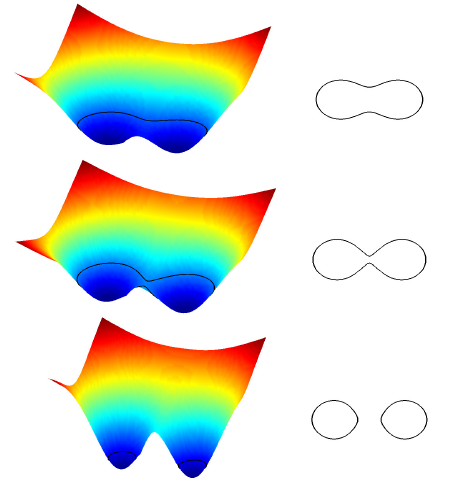
\includegraphics[scale=0.4]{images/levelsets.png}
		\caption{The relationship between the level set function (left) and contour (right) can be seen. It can be seen evolving the surface splits the contour.}
		\label{fig:levelsets}
	\end{figure}

The evolution of the contour or surface is governed by a level set equation. The solution tended to by this partial differential equation is computed iteratively by updating $\phi$ at each time interval. The general form of the level set equation is shown below.

	\begin{equation}
	\frac{\partial{\phi}}{\partial{t}}=-|\nabla{\phi|}\cdot F
	\label{eq:levelsetequation}
	\end{equation}

In the above level set equation $F$ is the velocity term that describes the level set evolution. By manipulating $F$, we can converge the level set to different areas or shapes, given an initialisation of the level set function. 

\section{Segmentation using Level Sets}
Typically, for applications in image segmentation $F$ is dependent on the pixel intensity or curvature values. It may also be dependent on an edge indicator function, which is defined as having a value zero on an edge, and zero otherwise. This causes $F$ to slow the level set evolution when on an edge.

In \cite{Lefohn04astreaming} $F$ is dependent on a data term and a curvature term (with a weighting term between the two) for the purposes of image segmentation. Therefore, the level set equation takes the form

	\begin{equation}
	\frac{\partial{\phi}}{\partial{t}}=-|\nabla{\phi}|\left[\alpha D(\bar{x})  + (1-\alpha)\nabla \cdot{\frac{\nabla{\phi}}{|\nabla{\phi|}}}\right]
	\label{eq:fulllevelsetequation}
	\end{equation}

where the data function $D(I)$ tends the solution towards targeted features, and the mean curvature term $\nabla \cdot{(\nabla{\phi}/|\nabla{\phi|})}$ keeps the level set function smooth. Weighting between these two is $\alpha \in [0,1]$, a free parameter that is set beforehand to control how smooth the contour or surface should be.

The data function $D(I)$ acts as the principal 'force' that drives the segmentation. By making $D$ positive in desired regions or negative in undesired regions, the model will tend towards the segmentation sought after. A simple speed function that fulfills this purpose, used by Lefohn, Whitaker and Cates in \cite{Lefohn04astreaming, gist}, is given by

	\begin{equation}
	D(I)= \epsilon - |I-T|
	\label{eq:dataterm}
	\end{equation}

which is plotted in Figure \ref{fig:speedterm}. Here $T$ describes the central intensity value of the region to be segmented, and $\epsilon$ describes the intensity deviation around T that is part of the desired segmentation. Therefore if a pixel or voxel has an intensity value within the $T\pm\epsilon$ range the model will expand, and otherwise it will contract. 

	\begin{figure}[h]
		\centering
			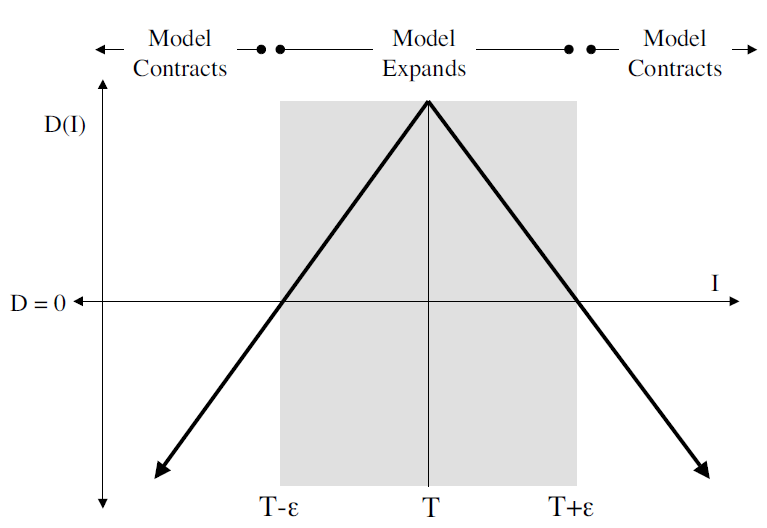
\includegraphics[scale=0.3]{images/speedterm.png}
		\caption{The speed term from \cite{gist}}
		\label{fig:speedterm}
	\end{figure}

Therefore the three user parameters that need to be specified for segmentation are $T$,$\epsilon$ and $\alpha$. An initialization for the level set function is also required, which may take the form of a cube in three dimensions or a square in two dimensions, or any other arbitrary closed shape. 

PICTURE OF CURVATURE FAIL


	\subsection{Signed Distance Transform}
A distance transform assigns a value for every pixel (or voxel) within a binary image containing one or more objects the value of which represents the minimum distance from that pixel to the closest pixel on the boundary of the object(s). The mathematical definition of a distance function $D:\mathbb{R}^3 \rightarrow \mathbb{R}$ for a set $S$, from \cite{oshersethian}, is
	
	\begin{equation}
	D(r,S) = \textrm{min}{|r-S|} \textrm{ for all } r \in \mathbb{R}^3
	\label{eq:distancetransform}
	\end{equation}

A \textit{signed} distance transform assigns the sign of the distance value as positive for those pixels outside the object, and negative for those inside it. It should be noted that the distance values depend on the chosen metric for distance: some common distance metrics are Euclidean distance, chessboard distance, and city block distance. Many of the algorithms that compute signed distance transforms often trade accuracy for efficiency and feature varying levels of complexity.

Signed distance transforms are required to initialize $\phi$ and also to reinitialize it every certain number of iterations. Computation of the initialization of $\phi$ is required before iteration of the level set equation can take place, and this will typically be a signed distance transform of an initial mask. Therefore the level set segmentation filter requires two images: an initial mask (which indicates targeted regions) and a \textit{feature} image (which is the image to be segmented). 
	
	\begin{figure}
	  \begin{center}
	    \subfigure[Arbitrary Initial Mask]{\label{fig:initmask}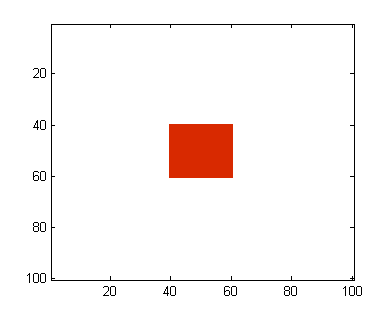
\includegraphics[scale=0.5]{images/initmask.png}}
	    \subfigure[Signed Distance Transform of Mask with Zero Level Set Overlaid]{\label{fig:sdf}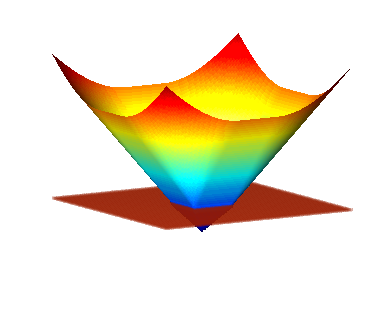
\includegraphics[scale=0.5]{images/sdf.png}}
	  \end{center}
	  \caption{2D Signed Euclidean Distance Transform}
	  \label{fig:sdfexplanation}
	\end{figure}


